\newpage
\section{Commandes}

		\subsection{Lancement du jeu}

		Au lancement de \emph{Bedbihan}, l'utilisateur peut débuter une nouvelle partie ou charger une partie préalablement sauvegardée. Le lancement d'une nouvelle partie implique de choisir une taille de carte et de sélectionner un peuple pour chacun des joueurs. Ceci est illustré par le diagramme d'utilisation de la {\sc Figure} \ref{fig:use1}.

		\begin{figure}
			\begin{center}
			%	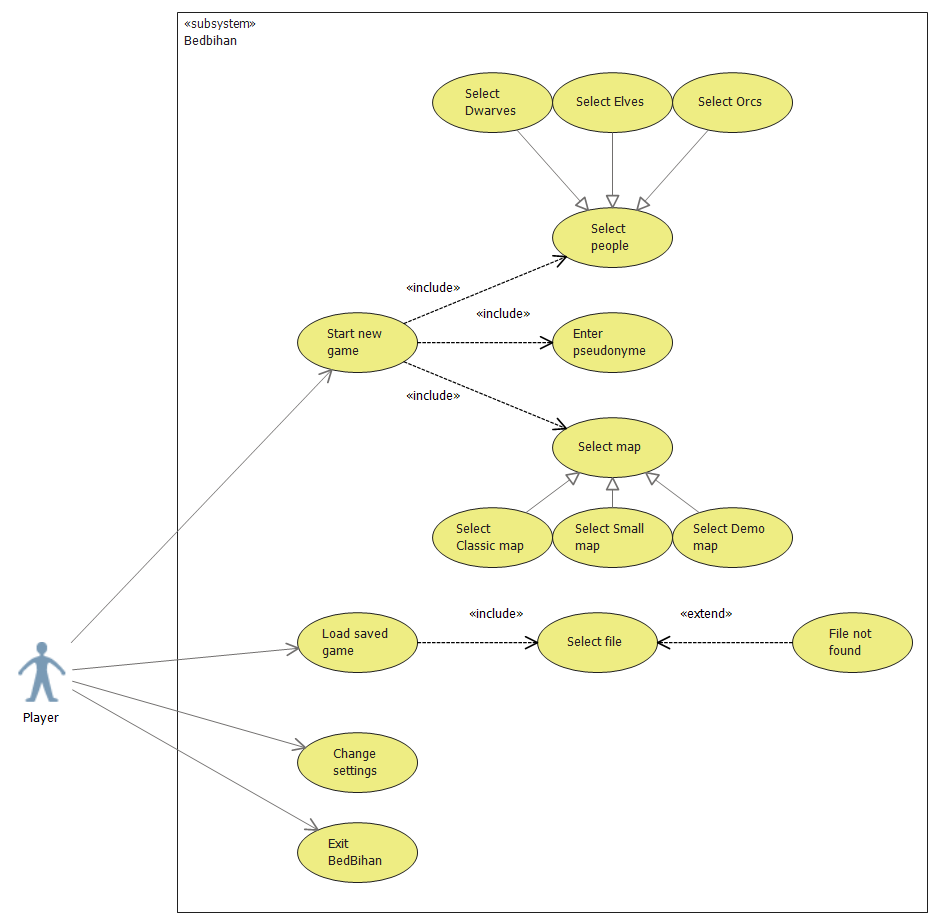
\includegraphics[width=1\textwidth]{figure/cas_utilisation_launch.png}
			\end{center}
			\caption{Actions possibles lors du démarrage du jeu.}
			\label{fig:use1}
		\end{figure}


	\subsection{Déroulement d'un tour}

		\emph{BedBihan} se jouant à tour de rôle, chaque tour se déroule comme illustré par le diagramme de séquence en {\sc Figure} \ref{fig:diagrammescouilles}. Chaque joueur dispose de différentes actions possible lorsque c'est à lui de jouer : ces différentes possibilités sont illustrées par le diagramme d'utilisation présenté en {\sc Figure} \ref{fig:use2}. Le déroulement séquentiel d'un tour pour un joueur est également illustré sur la {\sc Figure} \ref{fig:jetencule}
		